\documentclass[a4paper,landscape]{article}

\usepackage{amsmath}
\usepackage{pgfplots}

\def\USEJINJA{}

\ifdefined\USEJINJA
\def\rA{\VAR{rA}}
\def\tA{\VAR{tA}}
\def\rB{\VAR{rB}}
\def\tB{\VAR{tB}}
\def\version{\VAR{VERSION}}
\else
\def\rA{3}
\def\tA{45}
\def\rB{5}
\def\tB{90}
\def\version{template}
\fi  

\usetikzlibrary{shapes.misc, calc}

\pgfplotsset{compat=newest}

\def\ym{-6}
\def\yM{6}
\def\xm{-6}
\def\xM{6}

%\def\portrait{}

\ifdefined\portrait
  \def\H{29.7}
  \def\L{21.0}
\else
  \def\L{29.7}
  \def\H{21.0}
\fi


\newcommand{\millimetrique}[2]{
  \draw[step=1mm, line width=0.1mm, brown!25] (#1) grid (#2);
  \draw[step=5mm, line width=0.2mm, brown!50] (#1) grid (#2);
  \draw[step=1cm, line width=0.4mm, brown!75] (#1) grid (#2);
  \draw[step=5cm, line width=0.6mm, brown!100] (#1) grid (#2);
}

\newcommand{\logametrique}[6]{
  \coordinate (S) at ($(#3,#4)$) {};
  
  \foreach \i in {1,2} {
    \foreach \j in {1,...,9} {
      \coordinate (Q) at ($(0,0)!{log10(\i+(\j/10))}!(S)$) {};
      \draw[shift=(Q), xstep=#3cm,  ystep=#4cm, line width=0.2mm, #6!25]  ($(#1)+(0,2*#5)$) grid (#2);
    }
  }
  
  \foreach \i in {3,...,6} {
    \foreach \j in {2,4,...,8} {
      \coordinate (Q) at ($(0,0)!{log10(\i+(\j/10))}!(S)$) {};
      \draw[shift=(Q), xstep=#3cm, ystep=#4cm, line width=0.2mm, #6!25] ($(#1)+(0,1.5*#5)$) grid (#2);
    }
  }
  
  \foreach \i in {1,2,7,8,9} {
    \coordinate (P) at ($(0,0)!{log10(\i+0.5)}!(S)$) {};
    \draw[shift=(P), xstep=#3cm,  ystep=#4cm, line width=0.4mm, #6!50] ($(#1)+(0,#5)$) grid (#2);
  }
  
  \foreach \i in {2,...,9} {
    \coordinate (P) at ($(0,0)!{log10(\i)}!(S)$) {};
    \draw[shift=(P), xstep=#3cm, ystep=#4cm, line width=0.6mm, #6!75] ($(#1)+(0,0.5*#5)$) grid (#2);
  }
  \draw[xstep=#3cm, ystep=#4cm, line width=0.8mm, #6!100] (#1) grid (#2);
  % \draw[step=1mm, line width=0.1mm, #6!25] (#1) grid (#2);
  % \draw[step=5mm, line width=0.2mm, #6!50] (#1) grid (#2);
}

\newcommand{\cercle}[2]{
  \draw[fill=none, line width=0.6mm, brown!100](#1) circle (5) ;
  
  % \foreach \i [count=\k from 0] in {0,11.4591559026,...,359} {
  %
  \foreach \k in {0,...,31} {
    \draw ($(#1)+(#2+180/5/pi*\k:5.6)$) node[brown] {\textbf{\k}};
    \draw[line width=0.4mm, brown!100] ($(#1)+(#2+180/5/pi*\k:4.7)$) -- ($(#1)+(#2+180/5/pi*\k:5.3)$);
  }
  
  \foreach \k in {0,0.5,...,31} {
    \draw[line width=0.4mm, brown!100] ($(#1)+(#2+180/5/pi*\k:4.8)$) -- ($(#1)+(#2+180/5/pi*\k:5.2)$);
  }
  \foreach \k  in {0,0.1,...,31.4} {
    \draw[line width=0.2mm, brown!100] ($(#1)+(#2+180/5/pi*\k:4.9)$) -- ($(#1)+(#2+180/5/pi*\k:5.1)$);
  }
}

\begin{document}
\pagestyle{empty}

\begin{tikzpicture}[remember picture, overlay,  x=1cm, y=1cm]
  \coordinate (SW) at (current page.south west) ;
  \coordinate (NE) at (current page.north east) ;
  \coordinate (HD) at ($(NE) - (1.,1.)$);
  \coordinate (BG) at ($(SW) + (1.,1.)$);
  \coordinate (HG) at (BG |- HD);
  \coordinate (milieu) at ($(BG)!0.5!(HD)$);
  \coordinate (NG) at ($(BG)+(0,1)$);
  \coordinate (ND) at (HD |- NG);
  \coordinate (MG) at ($(NG)+(0,1)$);
  \coordinate (MD) at (HD |- MG);
  
  
  
  
%  \begin{scope}[shift={($(BG)+(3,3)$)}]
  \begin{scope}[shift=(milieu)]
    
    \millimetrique{MG}{HD}
    %\logametrique{BG}{MD}{10}{0}{0.8}{black} 
    
    \ifdefined\portrait
      \coordinate (centre) at ($(milieu) + (0.,5.)$);
      \draw[->] ($(centre)+(\xm,0)$) -- ($(centre)+(\xM,0)$) node[right] {$\mathcal{R}$};
      \draw[->] ($(centre)+(0,\ym)$) -- ($(centre)+(0,\yM)$) node[above] {$\mathcal{I}$};
    \cercle{centre}{0}
    \coordinate (A) at ($(centre)+(\tA:\rA)$); 
    \draw plot[mark=+] (A) node [ above right] {A};
    \coordinate (B) at ($(centre)+(\tB:\rB)$); 
    
    \else
      \coordinate (centre) at ($(milieu) + (-7.,0.)$);
      \draw[->] ($(centre)-(0,7)$) -- ($(centre)+(0,7)$) node[above] {$\mathcal{R}$};
      \draw[->] ($(centre)+(6,0)$) -- ($(centre)-(6,0)$) node[left] {$\mathcal{I}$};
          \cercle{centre}{90}
      \coordinate (A) at ($(centre)+(\tA+90:\rA)$); 
      \draw plot[mark=+] (A) node [ above right] {A};
      \coordinate (B) at ($(centre)+(\tB+90:\rB)$); 

    \fi
    
    
    
    
    \node[right] at ($(HD)+(-2,0.5)$){Calque ULAtrice};
    \node[right] at ($(BG)+(-0.5,-0.5)$){ULA: Uniform Log Arithmetic};
    \node[right] at ($(BG)+(23,-0.5)$){Utilise les  Logs Andouille ! (ULA)};

      \draw plot[mark=+] (A) node [ above right] {A};
      \draw plot[mark=+] (B) node [ above right] {B};

      \node[draw, right] at ($(MG)+(0,-0.3)$){\large{$\check{A}= \ldots + i. \ldots = \ldots.e^{i\,\ldots\;}$}};
      \node[draw, right] at ($(MG)+(0,-1)$){\large{$s_A(t) = \dots . \cos\left(\omega.t+\ldots\right)$}};
      \node[draw, right] at ($(MG)+(0,-1.7)$){\large{$s_A(t) = \dots . \cos\left(\omega.t\right)+\dots . \sin\left(\omega.t\right)$}};
      \node[draw, right] at ($(MD)+(-7,-0.3)$){\large{$\check{B}= \ldots + i. \ldots = \ldots.e^{i\,\ldots\;}$}};
      \node[draw, right] at ($(MD)+(-7,-1)$){\large{$s_B(t) = \dots . \cos\left(\omega.t+\ldots\right)$}};
      \node[draw, right] at ($(MD)+(-7,-1.7)$){\large{$s_B(t) = \dots . \cos\left(\omega.t\right)+\dots . \sin\left(\omega.t\right)$}};

    \node[right] at ($(milieu)+(-2.5,-10)$){\textbf{Pas de calculette !}};
    \node[right] at ($(HG)+(0,0.5)$){\version};


    
  \end{scope}
  
\end{tikzpicture}

\newpage
\pagestyle{empty}

\begin{tikzpicture}[remember picture, overlay,  x=1cm, y=1cm]
  \begin{scope}[shift={($(BG)+(1,2)$)}]
    
    \millimetrique{NG}{HD}{5}{5}
    %\logametrique{MG}{HD}{5}{5}{0}{brown}  
    \logametrique{BG}{ND}{10}{0}{0.3}{black}

    \node[right] at ($(HG)+(-0.5,0.5)$){Calque ULAtrice};
    \node[draw, right] at ($(milieu)+(-12.5,+8.4)$){\large{$\frac{\check{A}}{\check{B}}$ ou $\frac{\check{B}}{\check{A}} =  \underbrace{\ldots}_{\text{gain}}.e^{i\,\overbrace{\ldots^{ }\;}^{\text{déphasage [rad]}}}$}};

    \node[draw, right] at ($(milieu)+( -2.5,+8.4)$){\large{Gain de puissances~:$\frac{\left|\check{A}\right|^2}{\left|\check{B}\right|^2}=\quad\quad\quad$\textbf{en dB} ET l'inverse $\frac{\left|\check{B}\right|^2}{\left|\check{A}\right|^2}=\quad\quad\quad$ \textbf{en Bell !}}};
    
    \node[right] at ($(milieu)+(-12.5,7)$){Calculez la division avec Thalès au centième près~; avec un compas et l'échelle Log ci-dessous. Calculez une soustraction avec un compas et l'échelle linéaire};

    \node[right] at ($(milieu)+(-2.5,+10)$){\textbf{Pas de calculette ! Utiliser l'échelle log du bas}};
    \node[right] at ($(HD)+(-4,0.5)$){\version};

    \coordinate (Deux) at ($(13,0)$); 
    \coordinate (Un) at ($(10,0)$); 
    \coordinate (Dix) at ($(20,0)$); 
    \node at (Deux)  [ above] {${Log}_{10}(2)\approx 0,3$};
    \draw plot[mark=+] (Deux) node [below]{$3dB$};
    \node[] at ($(Deux)+(0,-2)$){$\times 2$};

     \draw[->] (-0.5,0) -- (25.5,0) node[right] {dB};
    \draw plot[mark=+] (Un) node [below]{$0dB$};
    \node[] at ($(Deux)+(-3,-2.3)$){$\times 1$};
    \draw plot[mark=+] (Dix) node [below]{$10dB$};
    \node[] at ($(Deux)+(7,-2.3)$){$\times 10$};
    
\end{scope}


\end{tikzpicture}

\end{document}
